\section{Обзор и классификация методов}

\begin{frame}{Два подхода к понижению размерности}
    \textbf{Отбор признаков:}
    \begin{itemize}
        \item Выбор подмножества исходных признаков.
        \item Сохранение информации без преобразования данных.
    \end{itemize}

    \textbf{Преобразование признаков:}
    \begin{itemize}
        \item Трансформация данных в новое пространство меньшей размерности.
        \item Сохраняет наиболее значимые свойства данных.
    \end{itemize}

    \begin{figure}
        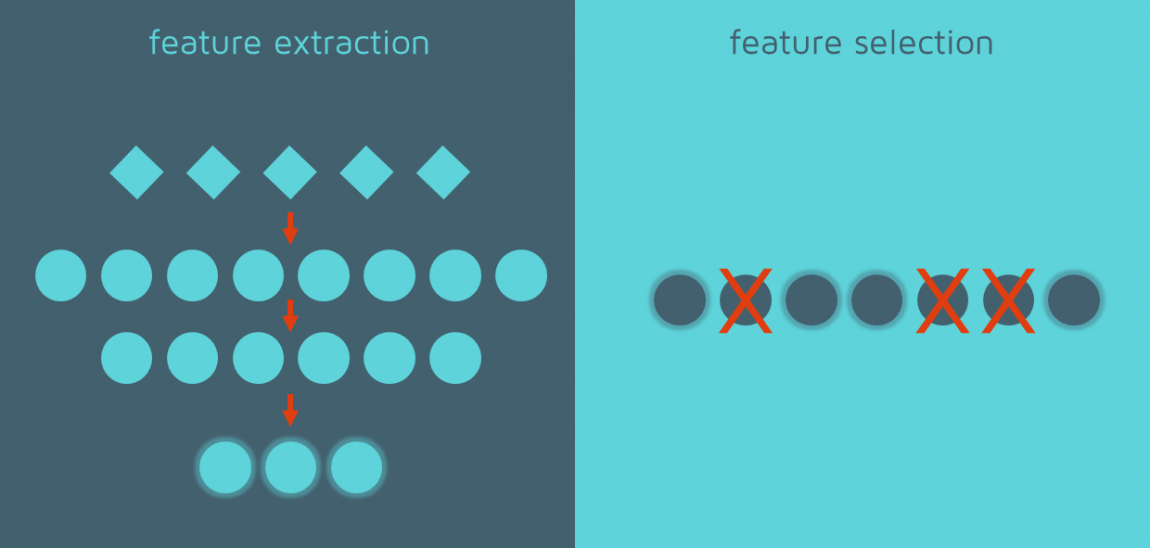
\includegraphics[width=.5\textwidth]{../resources/methods/feature_selection_vs_extraction.png}
    \end{figure}
\end{frame}

\begin{frame}
    \frametitle{Линейные методы}
    \begin{columns}
        \column{.6\textwidth}
        \begin{itemize}
            \item Предполагают, что данные лежат в \textbf{линейном подпространстве}.
            \item Преобразуют данные с помощью \textbf{линейных операций}.
        \end{itemize}
        \column{.6\textwidth}
        \begin{center}
            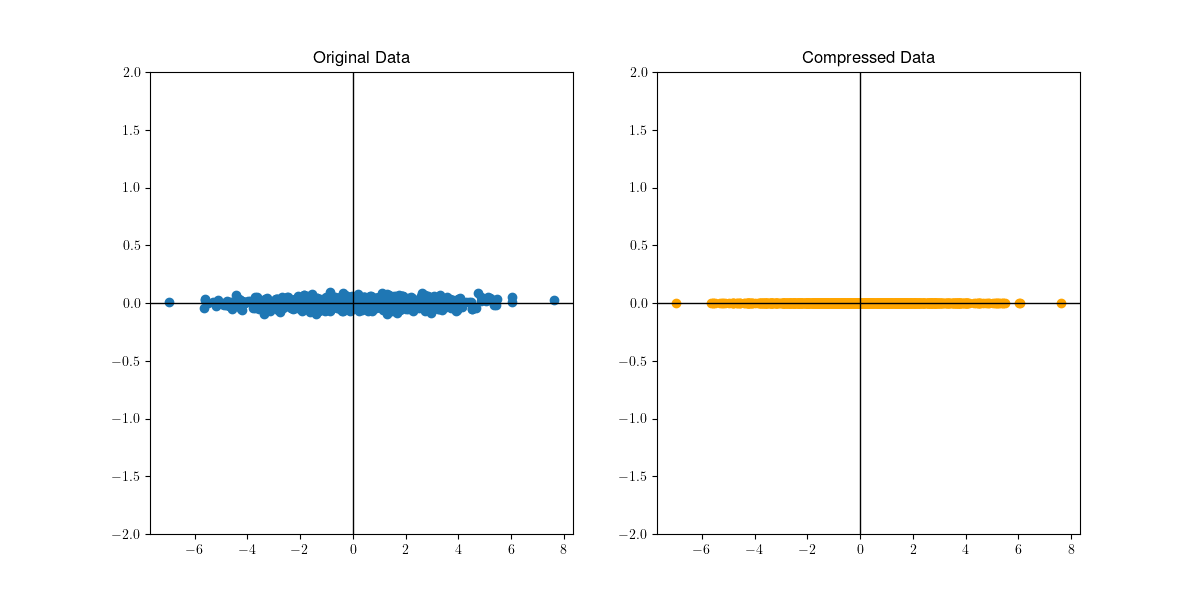
\includegraphics[width=.9\textwidth]{../resources/pca/simple_example_both.png}
            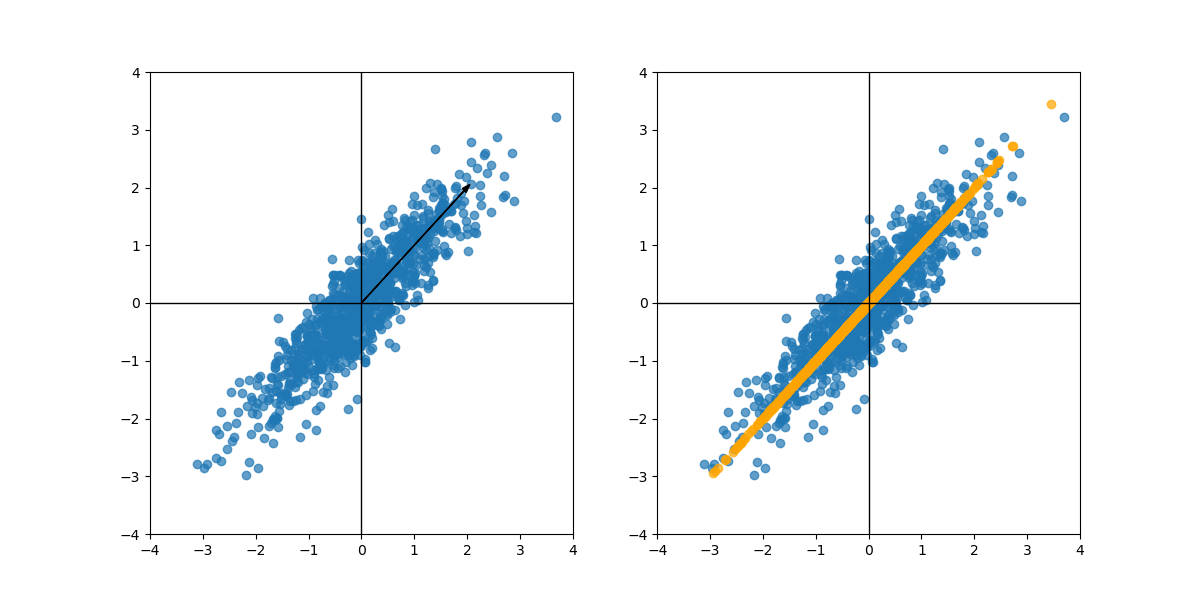
\includegraphics[width=.9\textwidth]{../resources/methods/pca.png}
        \end{center}
    \end{columns}
\end{frame}

\begin{frame}
    \frametitle{Нелинейные методы}
    \begin{columns}
        \column{0.55\textwidth}
        \begin{itemize}
            \item Данные имеют \textbf{сложные взаимосвязи}, которые нельзя описать линейно.
            \item Методы выявляют \textbf{нелинейные структуры} и сворачивают их в более простую форму.
        \end{itemize}
        \column{0.55\textwidth}
        \begin{center}
            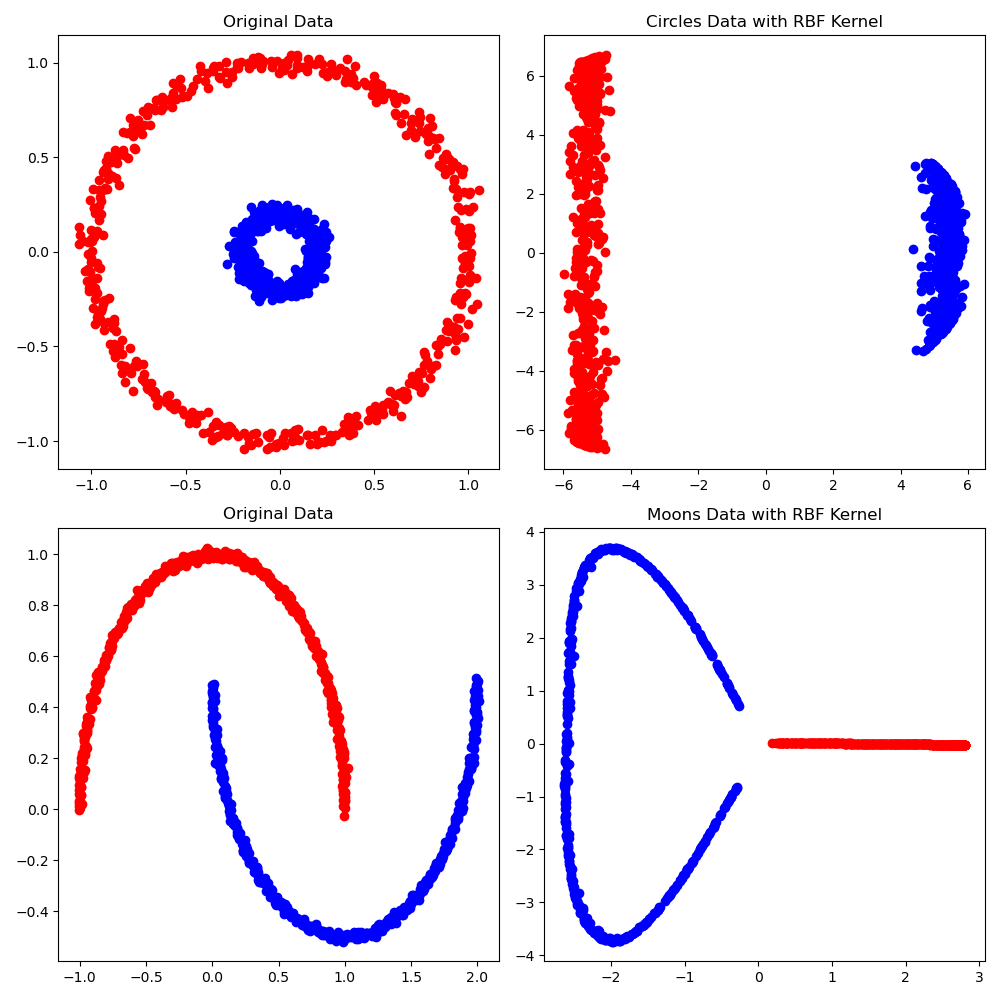
\includegraphics[width=1\textwidth]{../resources/methods/kpca.png}
        \end{center}
    \end{columns}
\end{frame}

\begin{frame}[allowframebreaks]{Principal Component Analysis (Анализ главных компонент, PCA)}
    \textbf{Основная идея:} Нахождение ортогональных направлений (главных компонент), вдоль которых дисперсия максимальна.

    \textbf{Ключевой момент:} Собственные векторы матрицы ковариации данных будут являться главными компонентами.

    \begin{center}
        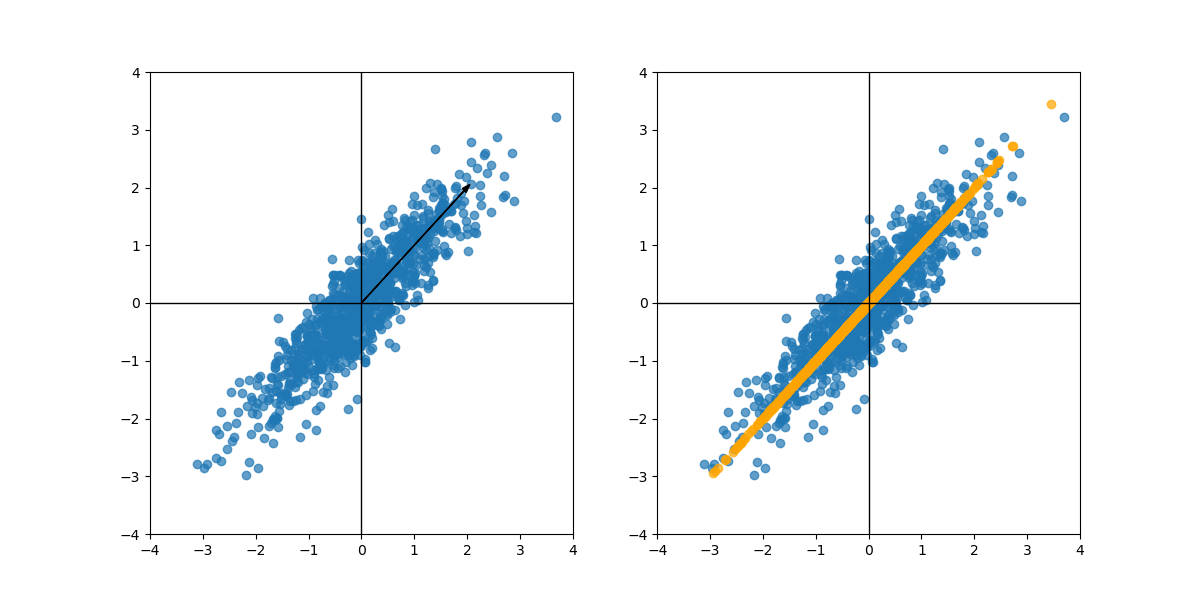
\includegraphics[width=.65\textwidth]{../resources/methods/pca.png}
    \end{center}

    \begin{center}
        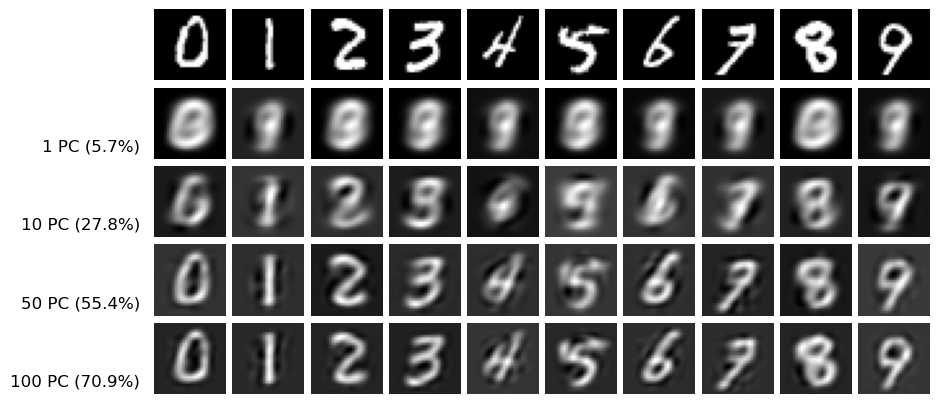
\includegraphics[width=1\textwidth]{../resources/pca/mnist_compression_demo.png}
    \end{center}

\end{frame}

\begin{frame}[allowframebreaks]{Kernel PCA (Ядерный PCA, KPCA)}
    \begin{columns}
        \column{0.5\textwidth}
        \textbf{Основная идея:} Применить PCA в пространстве более высокой размерности.

        \textbf{Ключевой момент:} Использование \textit{ядерного трюка} для избежания прямого преобразования данных в пространство высокой размерности.

        \column{0.55\textwidth}
        \begin{center}
            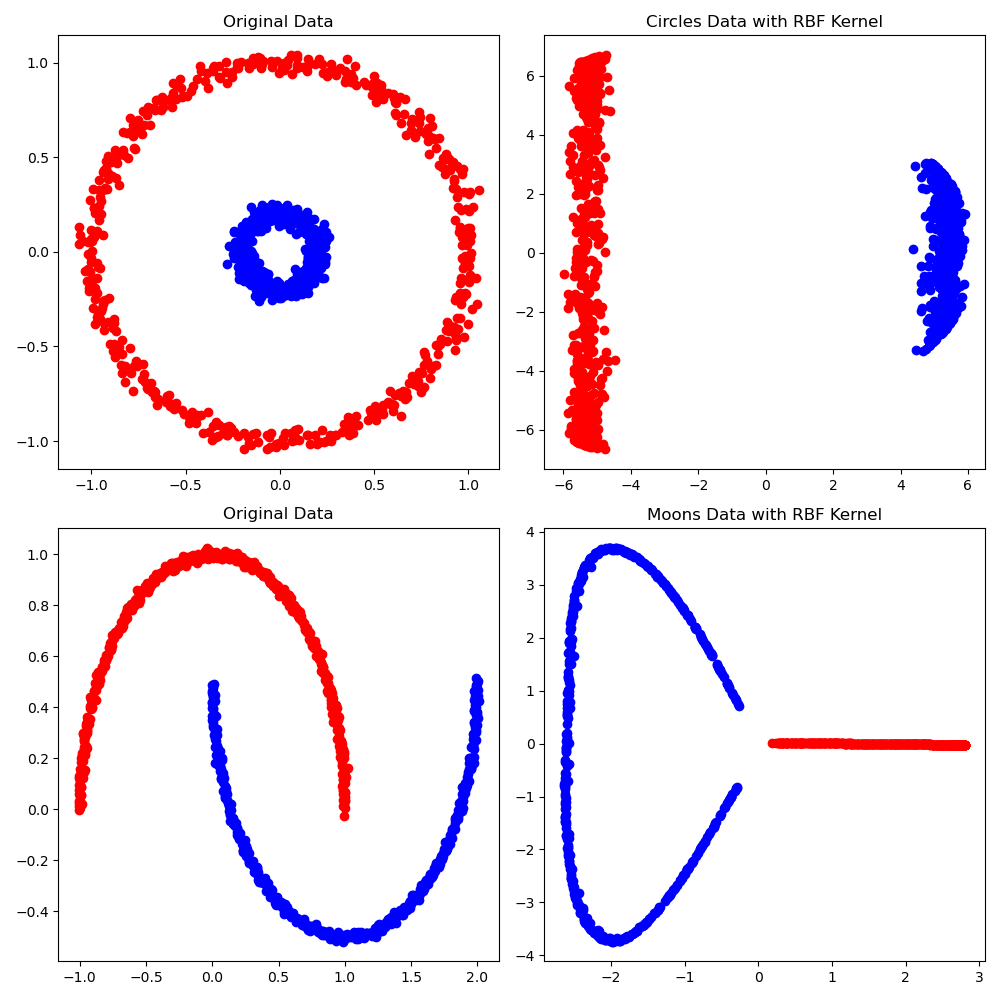
\includegraphics[width=1\textwidth]{../resources/methods/kpca.png}
        \end{center}
    \end{columns}

    \begin{columns}
        \column{0.55\textwidth}
        \begin{center}
            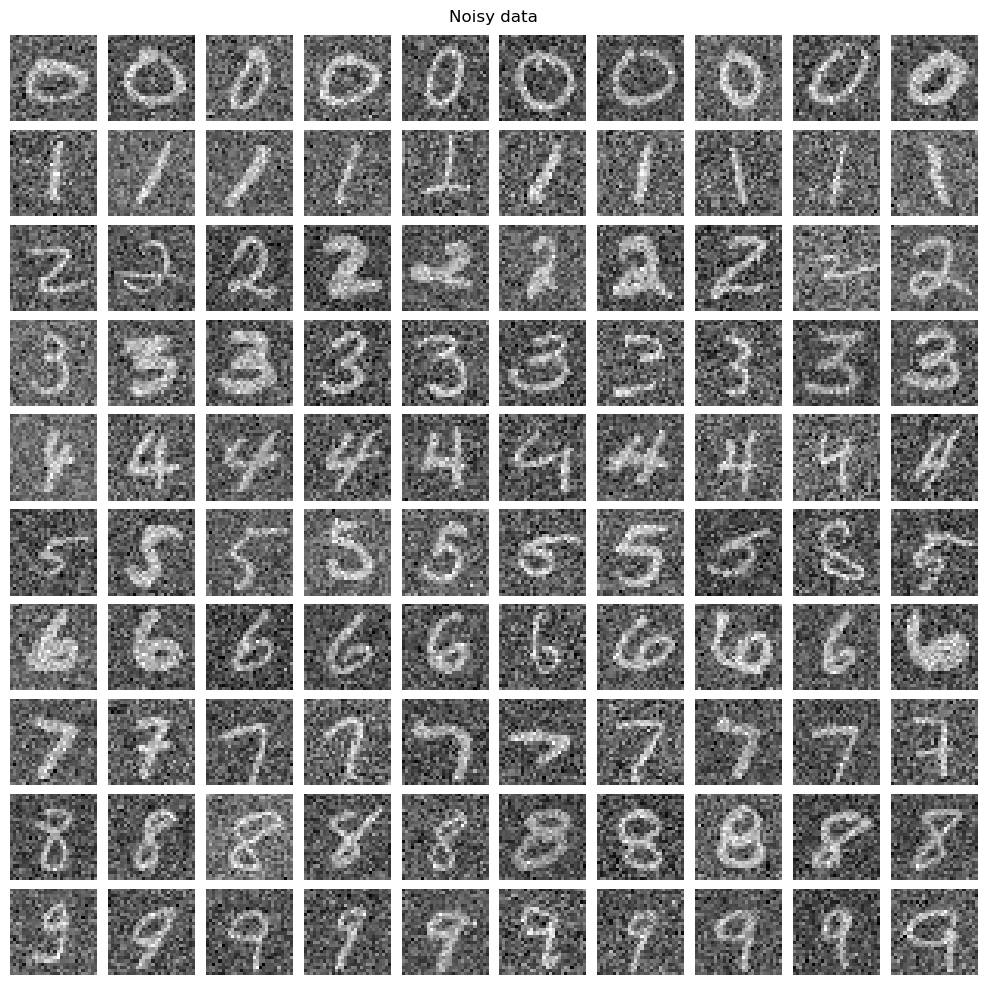
\includegraphics[width=1\textwidth]{../resources/kpca/mnist_noisy.png}
        \end{center}

        \column{0.55\textwidth}
        \begin{center}
            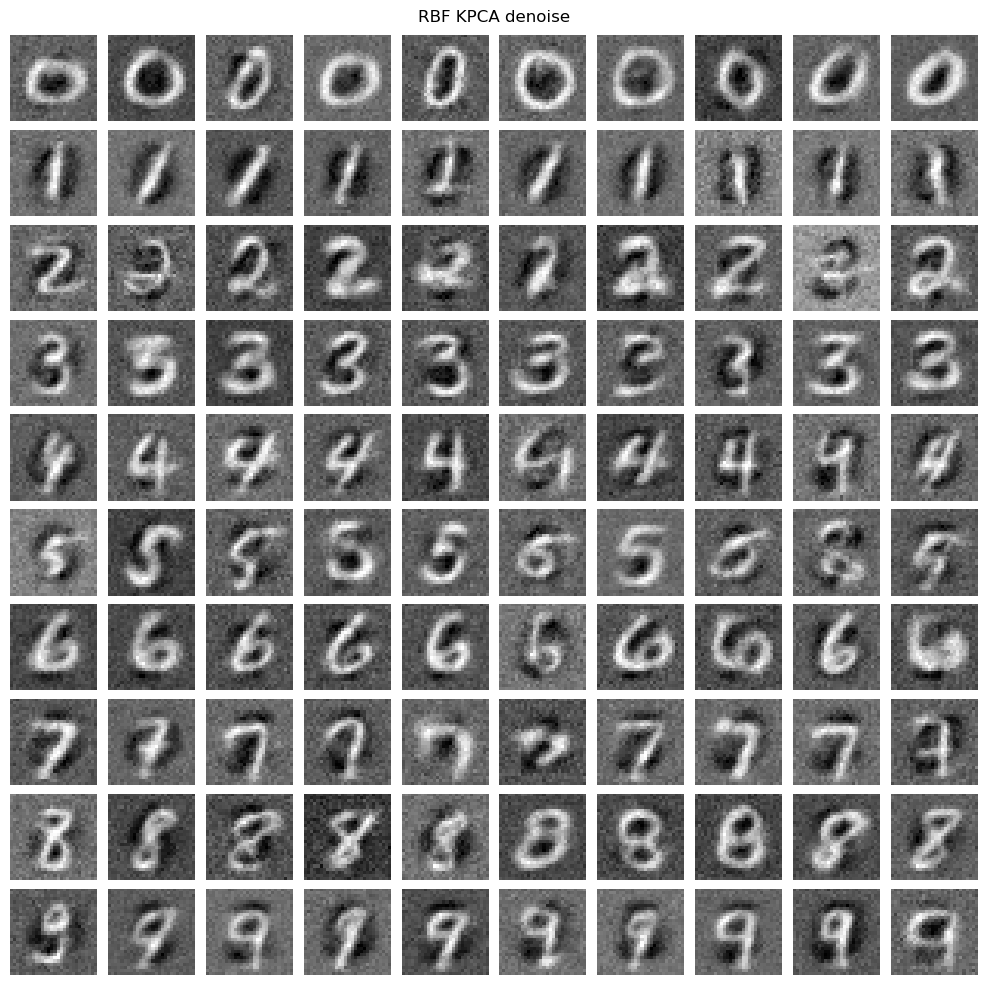
\includegraphics[width=1\textwidth]{../resources/kpca/mnist_denoise_kpca.png}
        \end{center}
    \end{columns}
\end{frame}

\begin{frame}[allowframebreaks]{AutoEncoders (AEs)}
    \textbf{Основная идея:} Нахождение компактных нелинейных представлений данных.

    \textbf{Ключевой момент:} Использование нейронных сетей, обучающихся восстанавливать входные данные, для построения нелинейных преобразований.

    \begin{columns}
        \column{0.55\textwidth}

        \textbf{Архитектура:}
        \begin{itemize}
            \item Кодировщик (encoder): преобразует входные данные в компактное представление.
            \item Декодировщик (decoder): восстанавливает данные из сжатого представления.
        \end{itemize}

        \column{0.45\textwidth}

        \begin{center}
            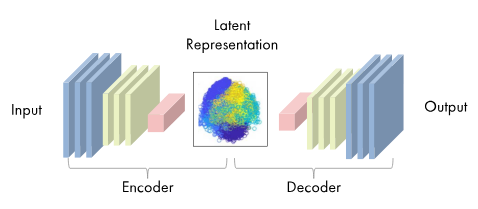
\includegraphics[width=1\textwidth]{../resources/methods/autoencoder.png}
        \end{center}
    \end{columns}

    \begin{columns}
        \column{0.55\textwidth}
        \begin{center}
            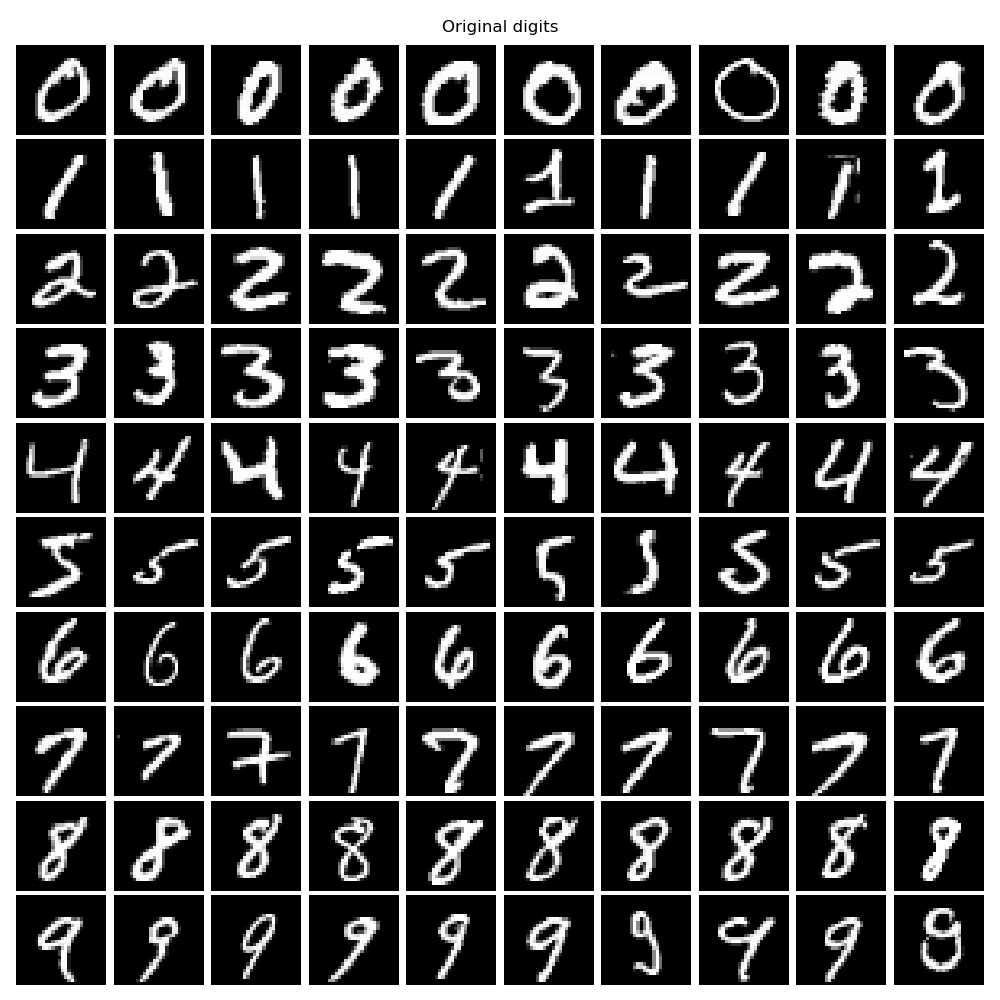
\includegraphics[width=1\textwidth]{../resources/ae/mnist_original_digits.png}
        \end{center}

        \column{0.55\textwidth}
        \begin{center}
            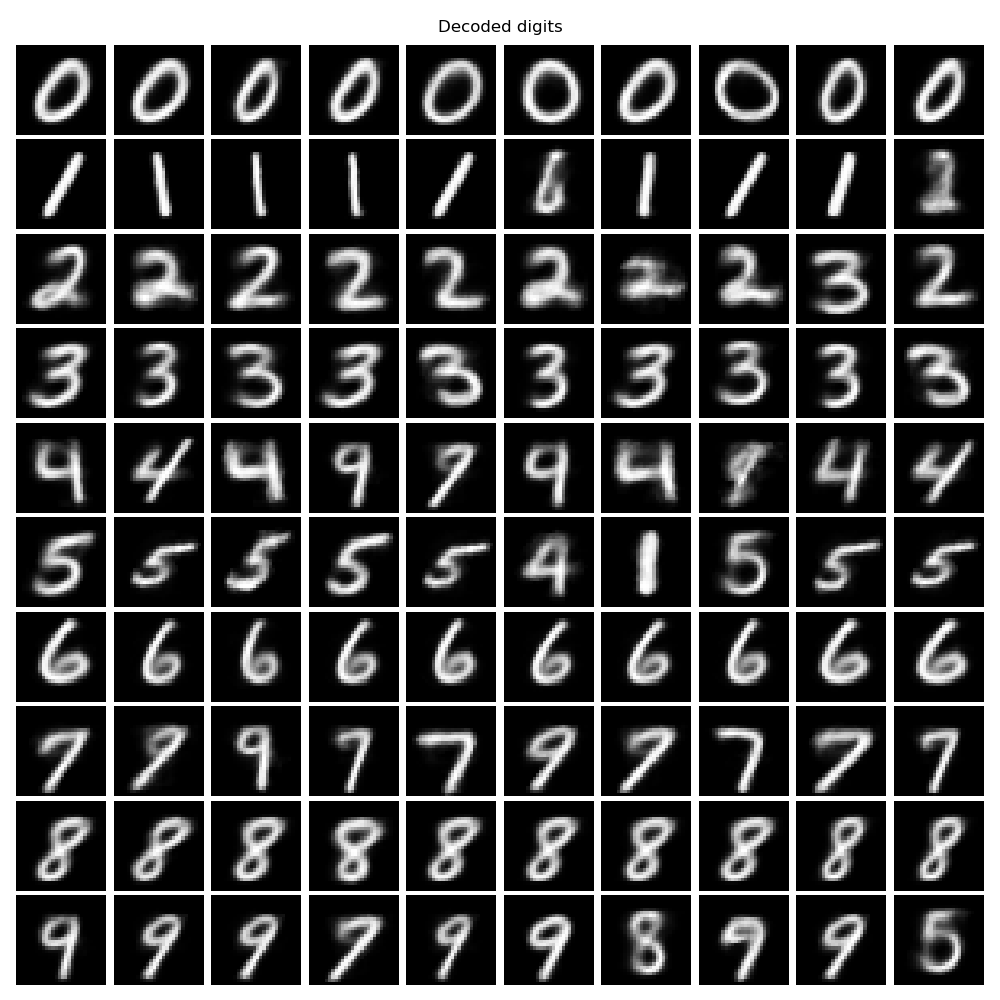
\includegraphics[width=1\textwidth]{../resources/ae/mnist_decoded_digits.png}
        \end{center}
    \end{columns}

    \begin{center}
        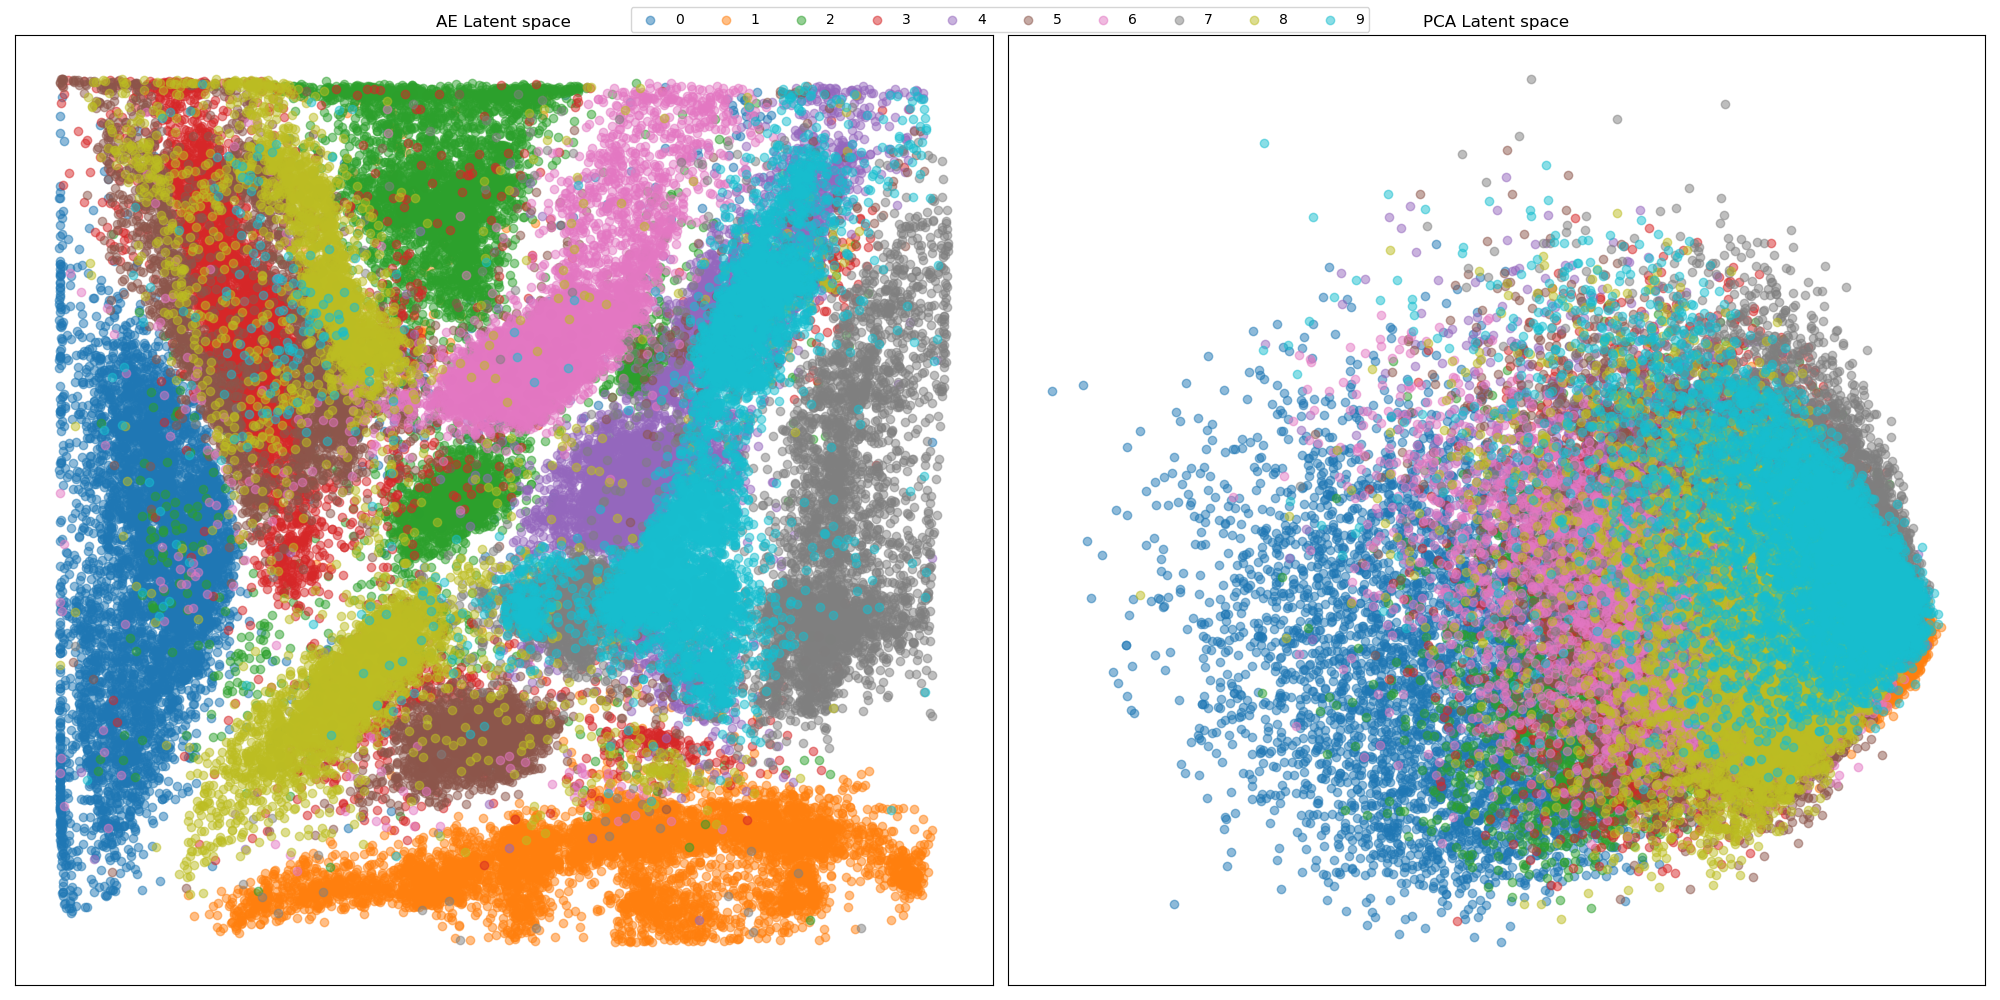
\includegraphics[width=1\textwidth]{../resources/ae/mnist_latent_spaces.png}
    \end{center}

    \begin{center}
        \begin{minipage}{0.32\textwidth}
            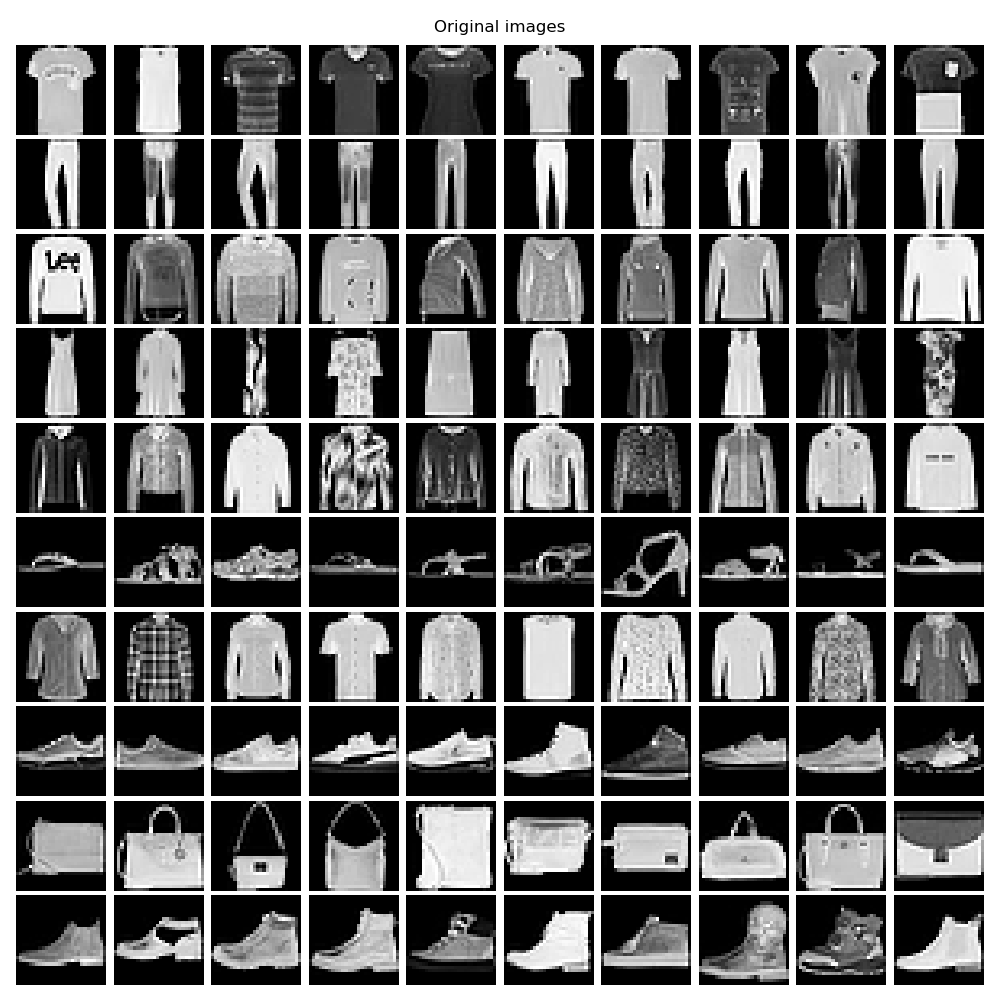
\includegraphics[width=\textwidth]{../resources/ae/fashion_mnist.png}
        \end{minipage}
        \begin{minipage}{0.32\textwidth}
            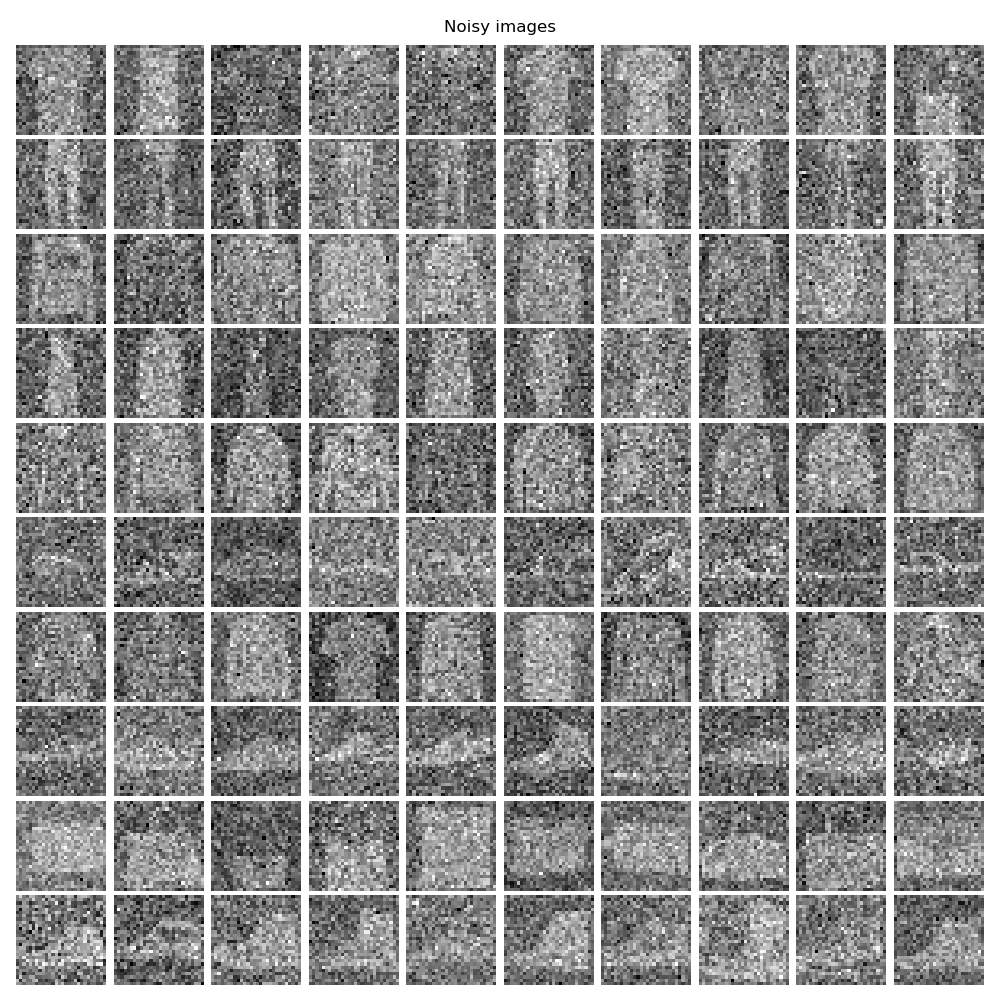
\includegraphics[width=\textwidth]{../resources/ae/fashion_mnist_noisy.png}
        \end{minipage}
        \begin{minipage}{0.32\textwidth}
            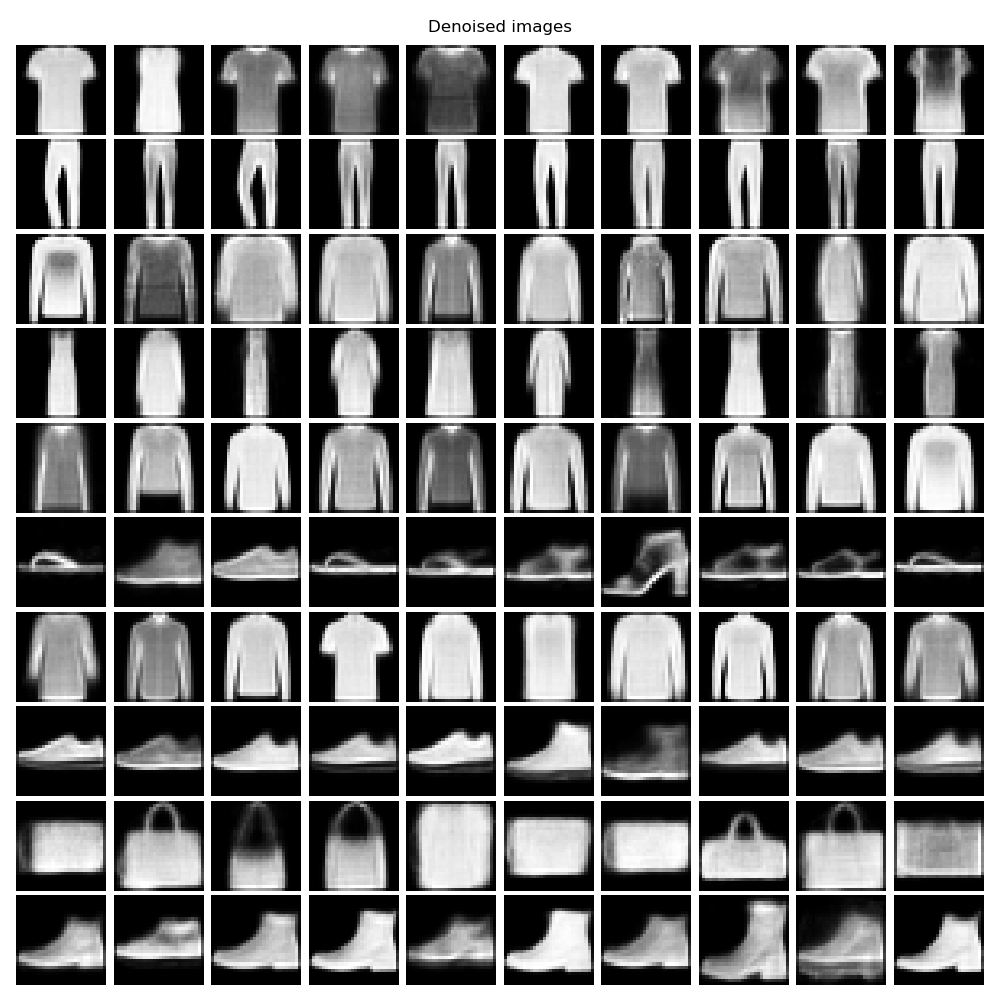
\includegraphics[width=\textwidth]{../resources/ae/fashion_mnist_denoised.png}
        \end{minipage}
    \end{center}
\end{frame}

\begin{frame}[allowframebreaks]{Variational AutoEncoders (VAEs)}
    \textbf{Основная идея: } Представление скрытого пространства в виде вероятностного распределения, что позволит генерировать новые данные.

    \begin{figure}
        \centering
        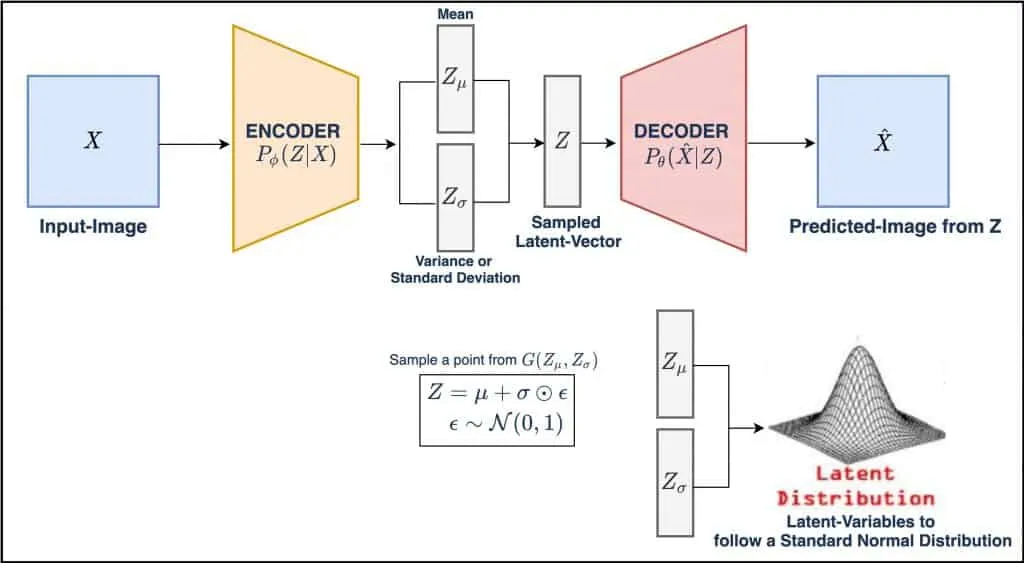
\includegraphics[width=0.6\textwidth]{../resources/methods/vae.png}
    \end{figure}

    \begin{columns}
        \column{0.55\textwidth}
        \begin{center}
            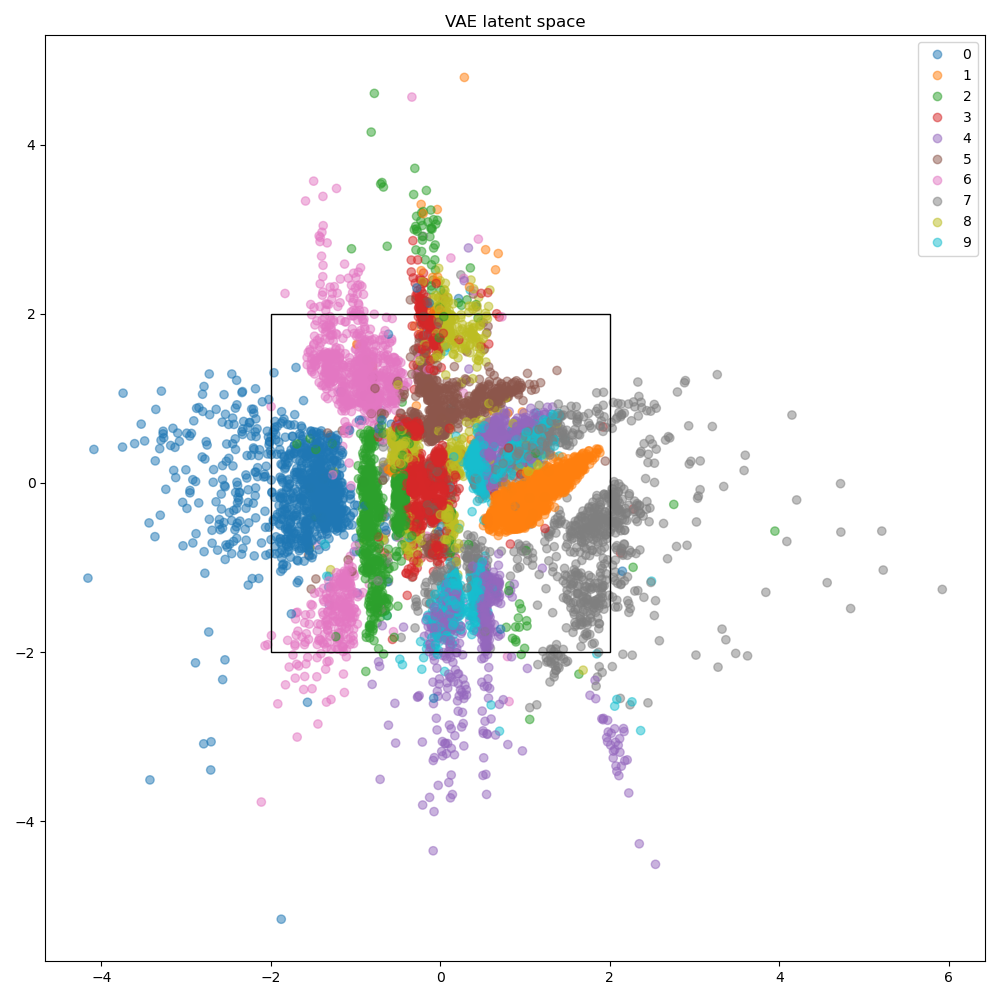
\includegraphics[width=1\textwidth]{../resources/vae/vae_latent_space_scatter.png}
        \end{center}

        \column{0.55\textwidth}
        \begin{center}
            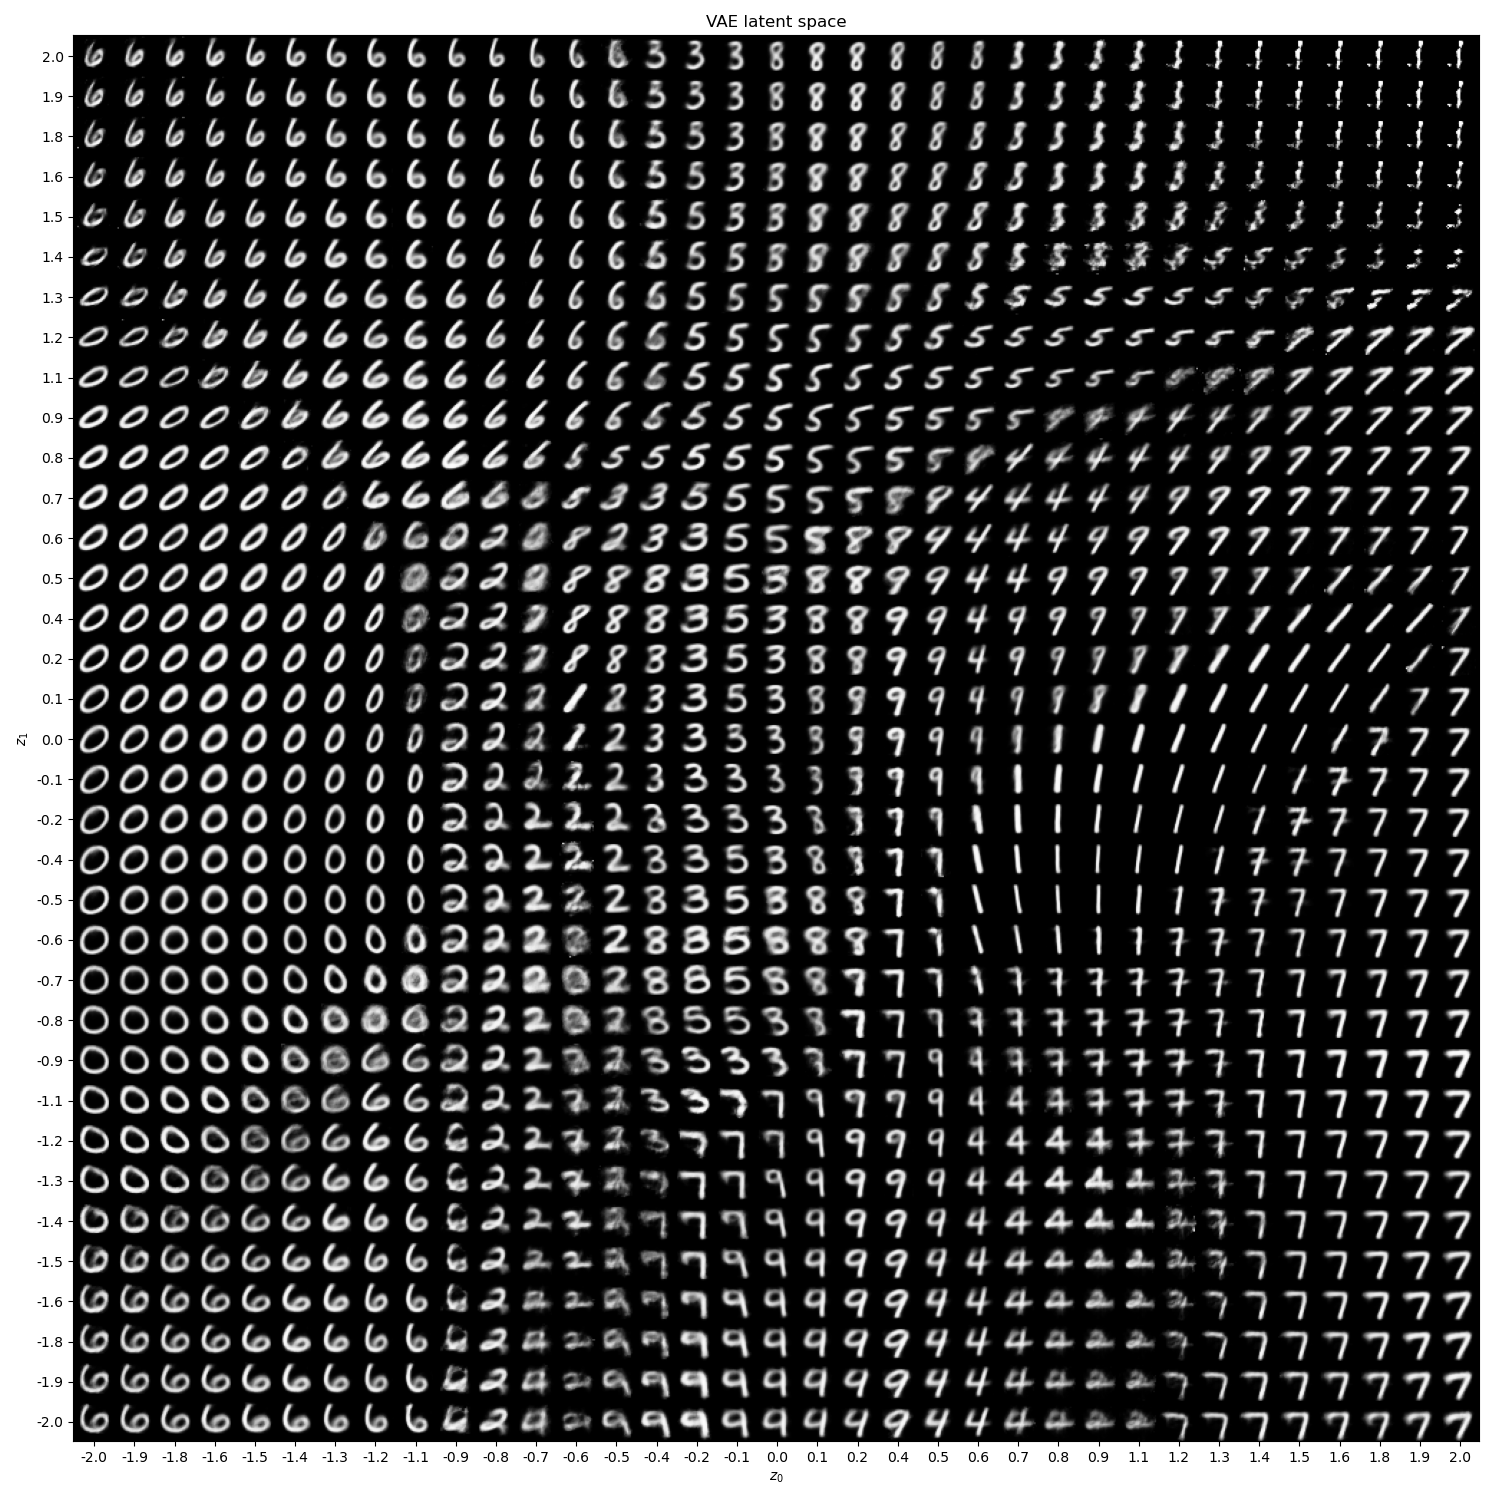
\includegraphics[width=1\textwidth]{../resources/vae/vae_latent_space_sample.png}
        \end{center}
    \end{columns}    
\end{frame}
